% Définition du répertoire contenant les images
\graphicspath{{IMAGE/}}

% FRAME Intro
\begin{frame}


\includegraphics[width=12cm]{Logos.pdf}

\vfill

\begin{center}

\vspace*{1.5cm}

\LARGE
\textbf{Concentration, Segregation, Autocorrelation}

\vspace*{1.5cm}
 DELHI GIS-R School


\large
9-12\up{th} April 2019

\vspace*{1.5cm}


\textbf{Hadrien Commenges \& Paul Chapron}

{\small

\vspace*{0.1cm}

\url{hadrien.commenges@univ-paris1.fr}

\url{paul.chapron@ign.fr}
}

\end{center}

\end{frame}

% FRAME
\begin{frame}{Le centre de la concentration}

\textbf{Où chercher de l'information sur les outils et les méthodes?}

~

GeoDa Center for Geospatial Analysis and Computation (Luc Anselin)

\url{https://geodacenter.asu.edu}

~

$\rightarrow$ logiciels \emph{standalone} (GeoDa) + bibliothèques Python et R \\
$\rightarrow$ tutoriels, bibliographie, cours en ligne


\end{frame}


% FRAME
\begin{frame}{Concentration}

\textbf{Méthodes classiques en économie des inégalités}

\begin{figure}
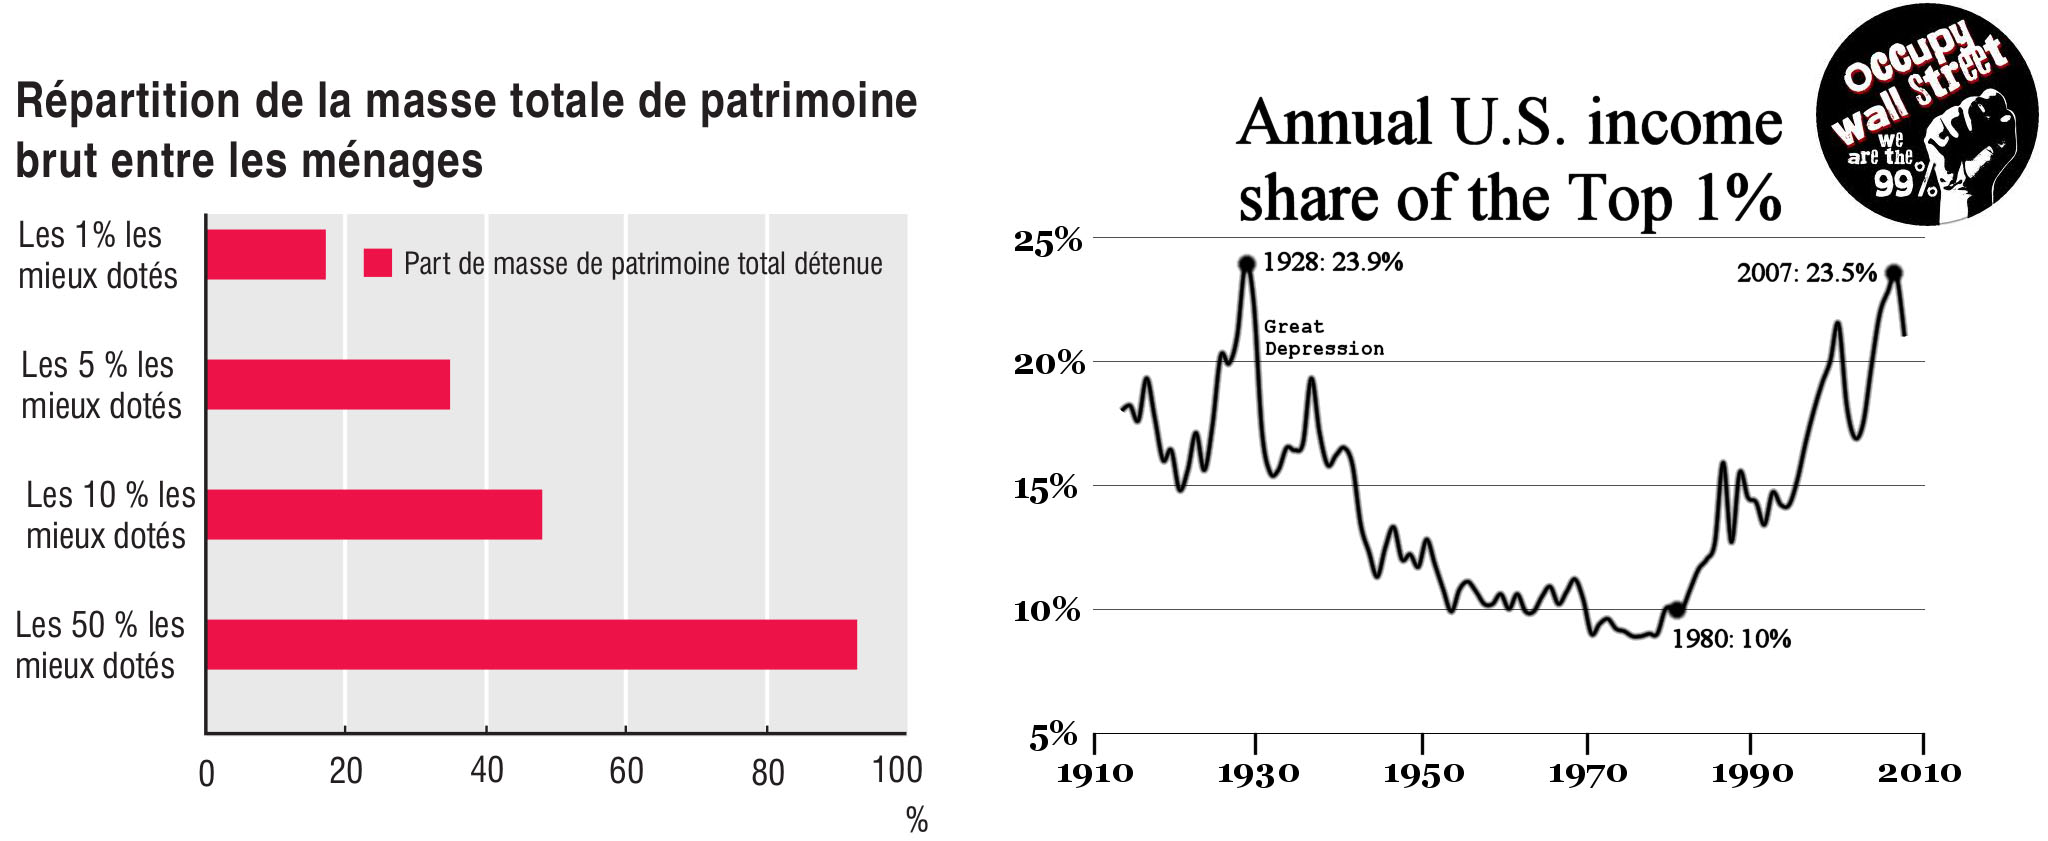
\includegraphics[width=12cm]{Inequalities.jpg}
\end{figure}

\end{frame}


% FRAME
\begin{frame}{Concentration}

\textbf{Indice de Hoover} \\
\emph{(Indice de dissimilarité} ou \emph{Indice de Duncan)}

~

Demi somme des différences absolues entre deux stocks:

\begin{equation}
\nonumber
H = \frac{1}{2} \sum_{i=1}^n \bigg| \frac{x_i}{x_{tot}} - \frac{y_i}{y_{tot}} \bigg|
\end{equation}

\end{frame}


% FRAME
\begin{frame}{Concentration}

\begin{figure}
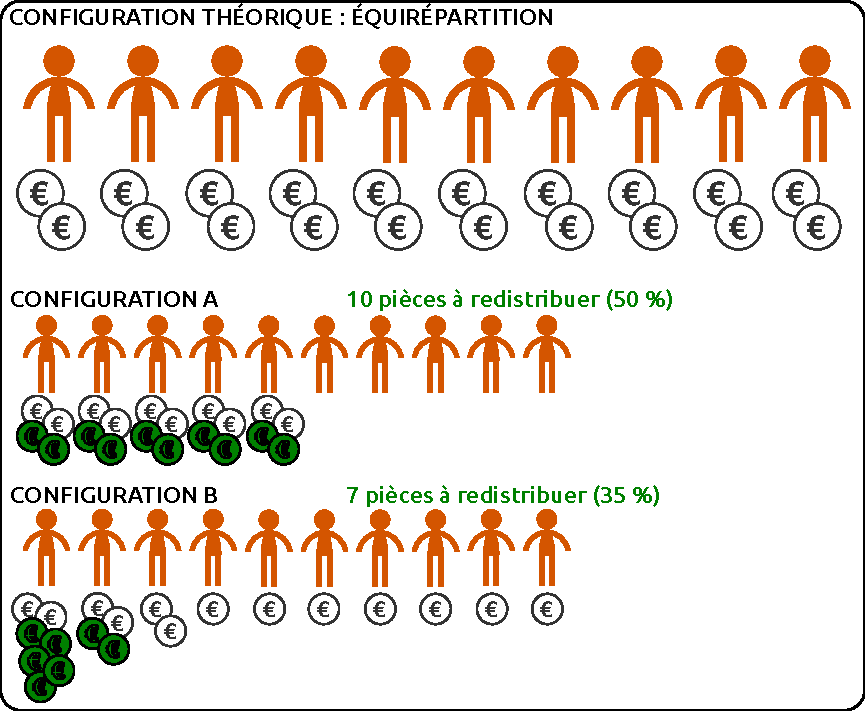
\includegraphics[width=9cm]{Gateau2.pdf}
\end{figure}

\end{frame}



% FRAME
\begin{frame}{Concentration}

\textbf{Indice de Gini}

~

Moyenne relative des différences absolues entre toutes les paires d'unités pour un stock:

\begin{equation}
\nonumber
G = \frac{\sum_i \sum_j |x_i - x_j|}{2n \sum_i x_i}
\end{equation}

\end{frame}


% FRAME
\begin{frame}{Concentration}

\begin{figure}
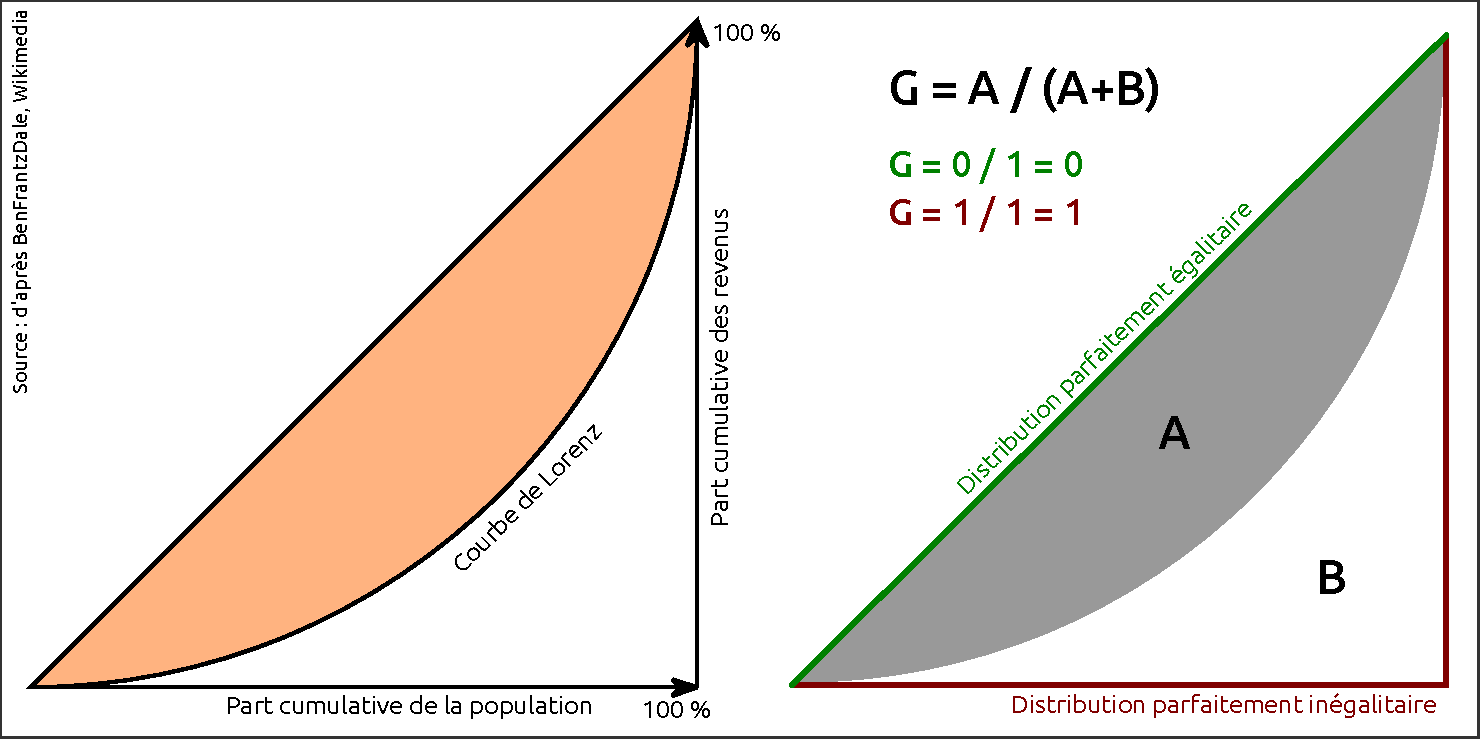
\includegraphics[width=12cm]{Lorenz.pdf}
\end{figure}

\end{frame}


% FRAME
\begin{frame}{Ségrégation}

\textbf{Mesures entropiques (théorie de l'information)}

~

\textbf{Quantité d'information:} logarithme (base 2) du quotient entre l'ensemble fini des évènements possibles avant information (N) et l'ensemble fini des évènements possibles après information (n):

\begin{equation}
\nonumber
  I = \log\left(\frac{N}{n} \right) = - \log(p)
\end{equation}

~

\textbf{Unité de cette quantité d'information:} le \textit{hartley}, le \textit{shannon} et surtout le \textit{bit} (\textit{binary digit})

\end{frame}


% FRAME
\begin{frame}{Ségrégation}

\textbf{Mesures entropiques (théorie de l'information)}

~ 

La mesure \textbf{I}: apparition d'un évènement informatif. 

La mesure \textbf{H} (entropie): information contenue dans un ensemble fini \\ 
- i.e. quantité d'information moyenne contenue dans un ensemble \\ 
- i.e. quantité d'information apportée par un évènement donné, multipliée par sa probabilité d'apparition

\begin{equation}
  H(x) = - \sum\limits_{i=1}^n p_i \log(p_i)
  \nonumber
\end{equation}

~

\textbf{Entropie relative:} rapport entre entropie observée et entropie maximale

\begin{equation}
  H_{max} = \log(n)
  \nonumber
\end{equation}

\end{frame}


% FRAME
\begin{frame}{Autocorrélation}

Hoover, Gini, Shannon (Theil) ne distinguent pas ces trois configurations \\
$\rightarrow$ ce sont des mesures presque aspatiales

\begin{figure}
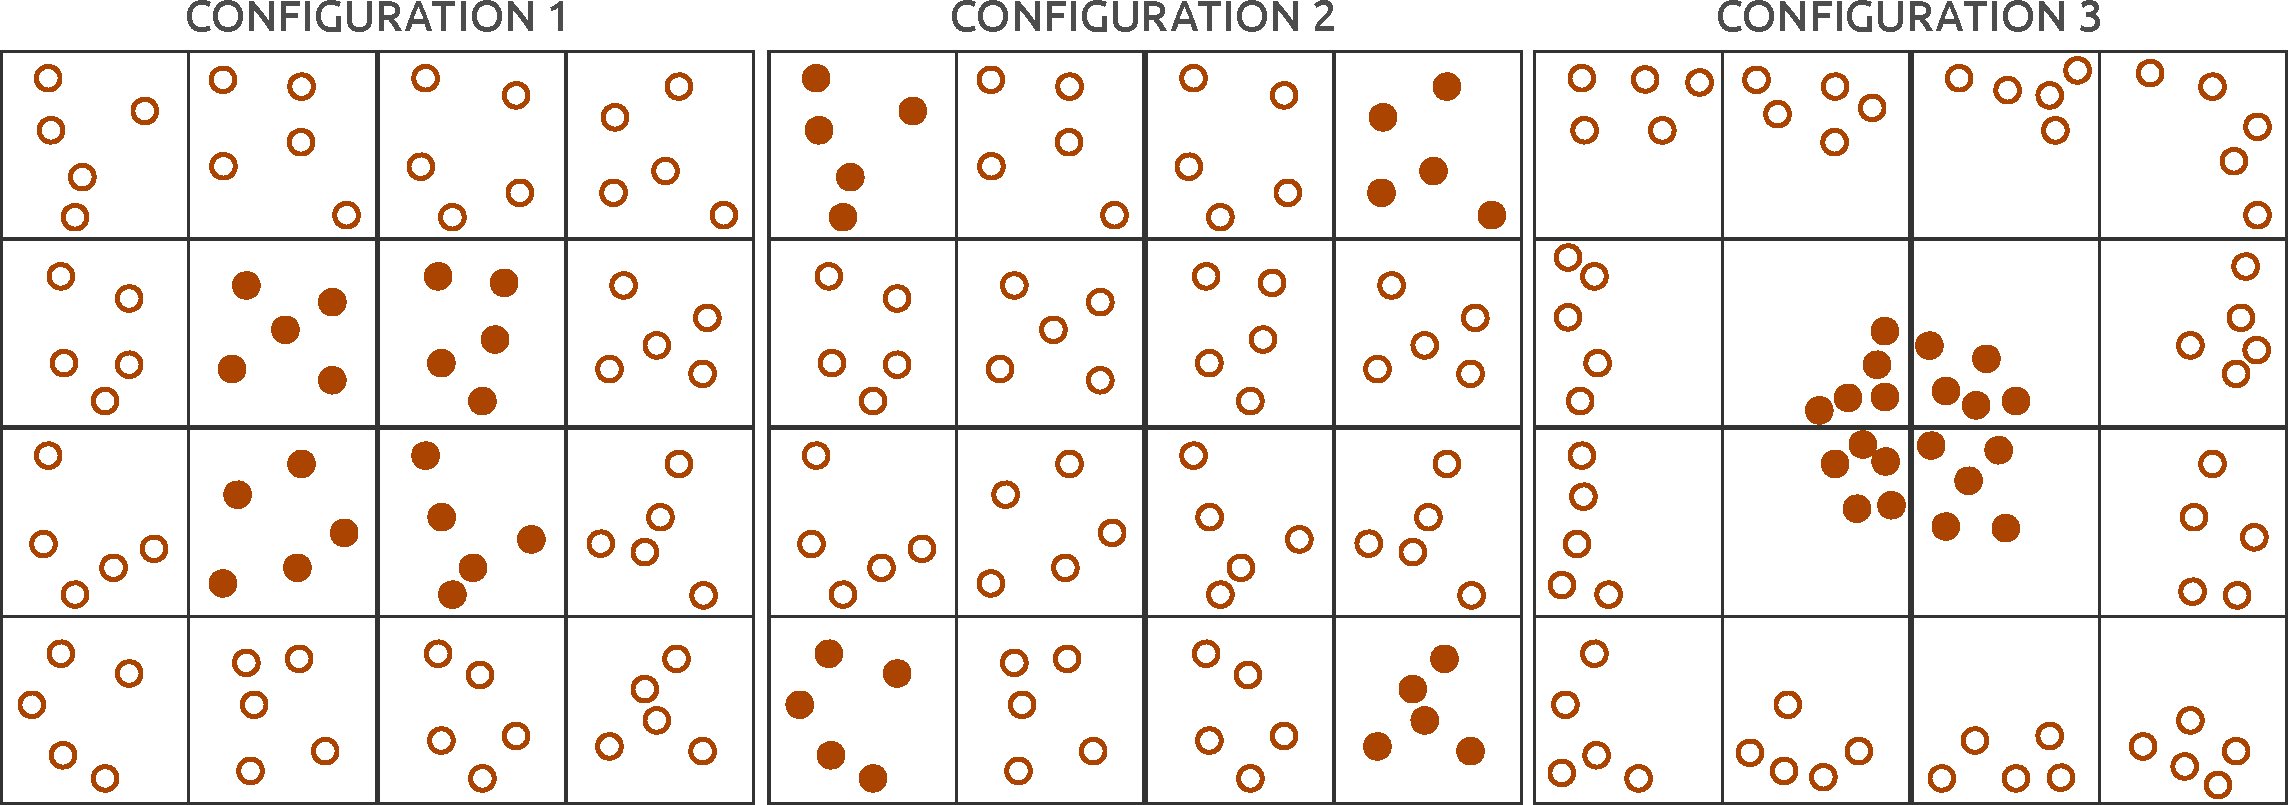
\includegraphics[width=12cm]{NonSpatial.pdf}
\end{figure}

Les méthodes d'autocorrélation (\textbf{Geary} et \textbf{Moran}) distinguent 1 et 2.

\end{frame}


% FRAME
\begin{frame}{Autocorrélation}

Indice \textbf{I} de Moran (1950):

$$
I = \frac{n}{\sum_{i} \sum_{j} w_{ij}} \times \frac{\sum_{i} \sum_{j} w_{ij} (x_i - \bar{x})(x_j - \bar{x})}{\sum_{i} (x_i - \bar{x})^2}
$$

~

$n$ : nombre d'individus \\ 
$x_i$ et $x_j$ : valeurs de la variable $x$ en $i$ et $j$ \\ 
$\bar{x}$ : moyenne de la variable $x$ \\ 
$w_{ij}$ : pondération correspondant à la définition du voisinage

\end{frame}



% FRAME
\begin{frame}{Autocorrélation}

Le graphique de Moran et son indice:

\begin{figure}
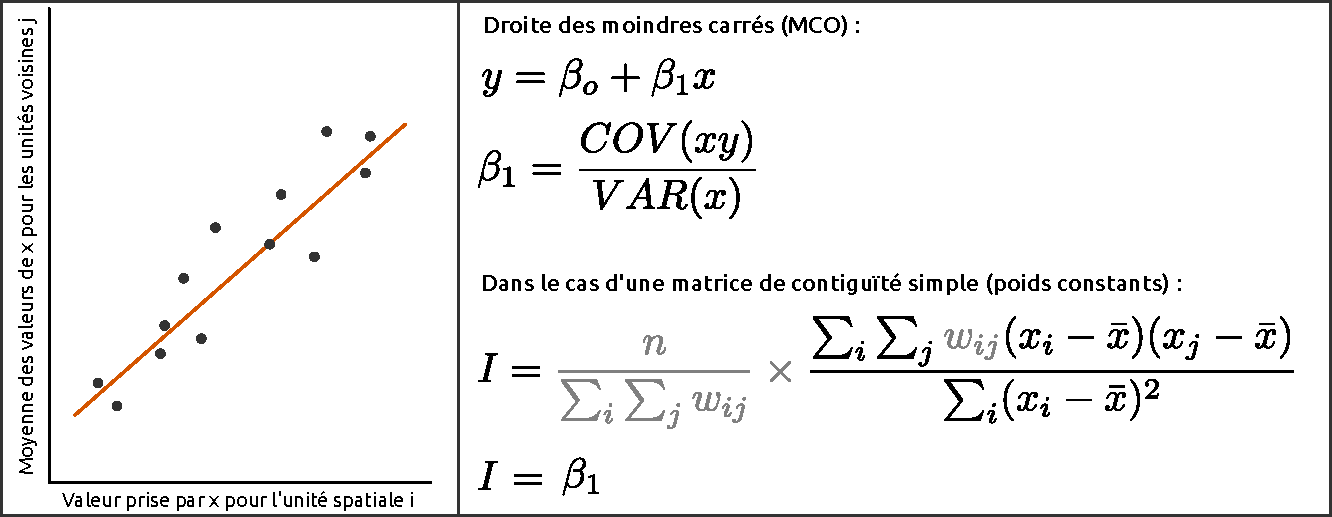
\includegraphics[width=12cm]{MoranPlot.pdf}
\end{figure}

\end{frame}


% FRAME
\begin{frame}{Autocorrélation}

\textbf{Contributions locales à la mesure globale d'autocorrélation} \\
LISA - \emph{local indicators of spatial autocorrelation}

$$
I_i = z_i \sum_{j} w_{ij} z_j
$$

~

$z_i$ valeur standardisée pour l'unité spatiale $i$ \\
$z_j$ valeur standardisée pour les unités voisines $j$ \\
$w_{ij}$ pondération par la matrice de contiguïté ou de poids

~

$\rightarrow$ \textbf{Moran plot:} nuage entre $x$ et moyenne de $x$ dans le voisinage

\end{frame}


% FRAME
\begin{frame}[fragile]{Application sur Paris}

\textbf{Charger les données:}

\begin{itemize}
  \item \texttt{dataParis}: données socio-éco dans les Iris parisiens
  \item \texttt{irisParis}: fond de carte correspondant (polygones)
\end{itemize}

~

\textbf{Exercices:}

\begin{itemize}
  \item Calculer l'indice de Hoover entre Français et étrangers
  \item Calculer l'indice de Gini sur les effectifs des différentes CSP
  \item Calculer l'entropie relative sur les CSP pour chaque Iris et cartographier l'indicateur
  \item Calculer l'autocorrélation entre cadres et ouvriers
\end{itemize}

~

\textbf{Packages nécessaires:} \texttt{spdep} pour l'autocorrélation, éventuellement \texttt{ineq} pour Gini, rien pour Hoover.

\end{frame}

